\documentclass[a4paper,11pt]{jsarticle}


% 数式
\usepackage{amsmath,amsfonts}
\usepackage{bm}
% 画像
\usepackage[dvipdfmx]{graphicx}
\bibliographystyle{myjunsrt}
\renewcommand{\bibname}{References}


\begin{document}

\title{}
\author{}
\date{\today}
\maketitle

\section{tangent delta}

The basic equation for electromagnetic waves
when there is loss in the medium is as follows

\begin{equation}
  \mathrm{rot}(\frac{1}{\mu(\boldsymbol{r})}\mathrm{rot}\boldsymbol{E}) = -\mu_0 \mathrm{rot}(\frac{\partial H}{\partial t})
\end{equation}
\begin{equation}
  \mathrm{rot}(\frac{\partial H}{\partial t}) = \epsilon(\boldsymbol{r})\epsilon_0 \frac{\partial^2 E}{\partial t^2} + \frac{\partial J}{\partial t}
\end{equation}


We consider the characteristic value when there is loss in the medium.
When we consider the incidence of the time-varying factor $exp(j\omega t)$,
Maxwell's Equation can be written as follows.

\begin{equation} \label{eq:loss_electric_flux_density}
  \mathrm{rot} H = \epsilon \epsilon_0 \frac{\partial E}{\partial t} + \sigma \boldsymbol{E} = (j\omega\epsilon\epsilon_0 + \sigma)\boldsymbol{E}
\end{equation}

In this case, the right-hand side of Equation \ref{eq:loss_electric_flux_density}
is considered to arise from the flux density $\boldsymbol{D}$.

\begin{equation} \label{eq:electric_flux_density}
  \boldsymbol{D} = C\epsilon \epsilon_0 \boldsymbol{E}(\boldsymbol{r})exp(j\omega t)
\end{equation}

We derive the constant $C=1 - j\sigma / \omega\epsilon\epsilon_0$ from the equation above.
Thus the electric flux density can be written as

\begin{equation} \label{eq:electric_flux_density_tangent_delta}
  \boldsymbol{D} = \dot{\epsilon} \epsilon_0 \boldsymbol{E} = \epsilon \epsilon_0 (1 - j\tan\delta)\boldsymbol{E}
\end{equation}

\begin{equation} \label{eq:epsilon_dot}
  \dot{\epsilon} = \epsilon (1 - j\tan\delta)
\end{equation}

\begin{equation} \label{eq:tangent_delta}
  \tan \delta = \frac{\sigma}{\omega\epsilon\epsilon_0}
\end{equation}

The parameter in Eq. \ref{eq:tangent_delta} is known as the loss tangent.
At high frequencies, the contribution of the real part of $\epsilon$ becomes larger,
while at low frequencies, the contribution of the imaginary part becomes larger.
In other words, it can be said that when an AC electric field is applied to a dielectric,
a part of its energy is the ratio that becomes heat.

\section{Skin effect}

In many of the experiments in this study, 
millimeter waves are blocked by copper plates.
The conductivity of the conductor $\sigma$ becomes very large,
and the amplitude damping constant $\alpha$ and the phase constant$\beta$
can be estimated as below.

\begin{equation}
  \alpha \approx \beta \approx \sqrt[]{\frac{\omega\mu\mu_0\sigma}{2}}
\end{equation}

This means that the attenuation of electromagnetic waves increases with increasing conductivity of $\sigma$
and the electromagnetic wave attenuates exponentially.
The depth δ at which the amplitude of the electromagnetic wave
at the surface is 1/e is called the skin depth, which can be expressed as below.

\begin{equation}
  \delta = \frac{1}{\alpha} = \sqrt[]{\frac{2}{\omega\mu\mu_0\sigma}}
\end{equation}

This indicates that the skin depth becomes shallower
as the frequency of the electromagnetic wave increases and the conductivity increases.
In this case, the current flows only near the surface of the copper plate,
which is called the skin effect.
The fact that current flows means that resistance exists,
and the skin resistance is written as follows.

\begin{equation}
  Re\{Z_W\} = \sqrt[]{\frac{\omega\mu\mu_0}{2}} = \frac{1}{\delta\sigma}
\end{equation}

Therefore copper plates can be used to effectively block millimeter waves.

\section{Snell's law}

At the boundary surfaces of different media, reflection and refraction of electromagnetic waves occur.
This is described by Snell's law.
This law can be derived using Maxwell's equations and boundary conditions.

The boundary plane of the medium is the x-y plane,
and the medium is uniform in the y direction within each region.
The relative permittivity and relative permeability are
$\dot{\epsilon_1}$ and $\mu_1$ for the first medium, and
$\dot{\epsilon_2}$ and $\mu_2$ for the second medium.
Let the complex permittivity in the presence of loss be
$i$ for each medium, so take values of 1 and 2, respectively.


\begin{equation}
  \dot{\epsilon_i} = \epsilon_i(1 - j\frac{\sigma_i}{\omega\epsilon_i\epsilon_0})
\end{equation}

Here $\sigma$ is the conductivity,
$\omega$ is the angular frequency of the electromagnetic wave,
$\epsilon$ is the dielectric constant when there is no loss, and
$\epsilon_0$ is the dielectric constant of vacuum.
The specific permeability $\mu$ is assumed to be a real number this time.
Here the magnitude of the wavenumber of each medium is as follows as $k$.
$c$ is the speed of light in vacuum.

\begin{equation}
  k_i = \frac{\omega\sqrt[]{\dot{\epsilon_i}\mu_i}}{c}
\end{equation}

Here we derive Snell's law using the TE wave as an example.
For TE waves,
the oscillation direction of the electric field is perpendicular to the surface,
and there is no electric field component in the direction of propagation.
Since the direction perpendicular to the surface is the y-axis,
its electric field is $E^i_y$ and can be written as follows:

\begin{equation}
  E^i_y = A_{iS}\exp[j(\omega t - \boldsymbol{k}_i\cdot\boldsymbol{r})]
\end{equation}

$A_{iS}$ is the electric field amplitude,
$\boldsymbol{k}_i$is the wavenumber vector in the medium, and
$\boldsymbol{r}$ is the position vector to an arbitrary point on the wavefront.
The subscript $i$ has three states,
where incident, transmitted, and reflected are denoted by i, t, and r, respectively.

\section{Total Reflection}

When an electromagnetic wave is incident on a sparse medium from a dense medium,
the refraction angle reaches 90 degrees before the incident angle
as the incident angle is gradually increased.
This phenomenon in which the incident electromagnetic wave
returns to the incident side after being reflected
at the boundary surface without being transmitted is called total reflection.

The transmitted field components of the TE wave at total reflection
can be written as follows.


\begin{equation}
  E^t_y = \exp[-j(\sqrt[]{\epsilon_1\mu_1}k_0\sin\theta_t)x]\exp\left(-\frac{z}{z_g}\right)
\end{equation}

\begin{equation}
  z_g = \frac{c}{\omega\sqrt[]{\epsilon_1\mu_1\sin^{2}\theta - \epsilon_2\mu_2}}
\end{equation}

$z_g$ represents the depth of penetration of the electric field into the second medium,
indicating that the electromagnetic wave is seeping slightly into the boundary surface.
Even during total reflection, 
electromagnetic waves also slightly penetrate to the other side of the boundary.
This component is called the evanescent wave.
Along with the penetration of the electromagnetic field,
the reflection point is also shifted.
This shift is called the Guschenchen shift.
This is important when using dielectric waveguides and optical fibers.


Electromagnetic waves do seep out slightly
to the other side of the boundary plane,
but it is important to note that the energy does not seep out.
It is important to note that energy does not seep out.
The sum of the amplitude reflection coefficients all add up to 1,
and all energy is also reflected.

\begin{figure}
  \begin{center}
    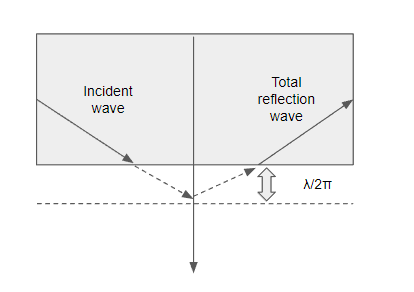
\includegraphics[clip, keepaspectratio, width=0.5\linewidth]{img/insertion_reflection_evanescence.png}
    \caption{evanescent成分の浸みだし}
    \label{fig:insertion_reflection_evanescent}
  \end{center}
\end{figure}


\section{Transmission loss of electromagnetic waves}

Transmission loss of an electromagnetic wave in free space
can be written as follows as $L$.

\begin{equation}
  L = \left(\frac{4\pi d}{\lambda} \right)^2
\end{equation}

Here $\lambda$ is the wave length, and $d$ is the distance.
At 28GHz, which has the wave length of 10mm,
the loss at the distance of 0.25cm can be computed as -49.3 decibels.
At 800MHz (wave length of 375mm), the same loss of -49.3 decibels can be seen at
the distance of 10 meters.

TODO:画像追加

\section{Link budget}

\section{Cutoff Frequency}

A cutoff frequency, corner frequency, or break frequency
is a boundary in a system's frequency respoonse at which
energy flowing through the system begins to be reduced
rather than passing through.
Cutoff frequency in a rectangular waveguide can be calculated as follows,
where $a$ is the wall length, and $\mu$ and $\epsilon$ are
the permeability and permittivity of the material
that fill the waveguide, respectively.

\begin{equation}
  f_c = \frac{1}{2a\sqrt[]{\mu\epsilon}}
\end{equation}

In a circular waveguide with radius of $a$,
this could be written as

\begin{equation}
  f_c = \frac{1.8412}{2\pi a\sqrt[]{\mu\epsilon}}
\end{equation}

\section{曲がるアンテナ}

先行研究として株式会社NTTドコモが開発した曲がるアンテナが存在する
\cite{bending_antenna}。

\newpage
\addcontentsline{toc}{chapter}{\bibname}
\bibliography{common_bibliography}

\end{document}